\documentclass[11pt,a4paper]{article}
\usepackage[utf8]{inputenc}
\usepackage[T1]{fontenc}
\usepackage{amsthm} %numéroter les questions
\usepackage[frenchb]{babel}
\usepackage{datetime}
\usepackage{xspace} % typographie IN
\usepackage{hyperref}% hyperliens
\usepackage[all]{hypcap} %lien pointe en haut des figures
\usepackage[french]{varioref} %voir x p y
\usepackage{fancyhdr}% en têtes
%\input cyracc.def
\usepackage[]{graphicx} %include pictures
\usepackage{pgfplots}
\usepackage[ ]{circuitikz}
\usepackage{ifthen}

\usepackage[top=1.3 in, bottom=1.3 in, left=1.3 in, right=1.3 in]{geometry} % Yeah, that's bad to play with margins
\usepackage[]{pdfpages}

\usepackage[]{attachfile}

\usepackage{float}

\newdateformat{mydate}{2016--2017}%hack pour remplacer \THEYEAR


\newboolean{corrige}
\ifx\correction\undefined
\setboolean{corrige}{false}% pas de corrigé
\else
\setboolean{corrige}{true}%corrigé
\fi

%\setboolean{corrige}{false}% pas de corrigé

\newboolean{annexes}
\setboolean{annexes}{true}%annexes
%\setboolean{annexes}{false}% pas de annexes

\definecolor{darkblue}{rgb}{0,0,0.5}

\newboolean{mos}
%\setboolean{mos}{true}%annexes
\setboolean{mos}{false}% pas de annexes

\usepackage{aeguill} %guillemets

%% fancy header & foot
\pagestyle{fancy}
%Numero du TP :
\def \labonumber {Labo \no 2 }
\lhead{[ELEC-H-310] Choucroute numérique\\ \labonumber}
\rhead{\mydate\today\\ page \thepage}
\chead{\ifthenelse{\boolean{corrige}}{Corrigé}{}}
\cfoot{}
%%

\pdfinfo{
/Author (Quentin Delhaye, Ken Hasselmann, ULB -- BEAMS)
/Title (\labonumber ELEC-H-310)
/ModDate (D:\pdfdate)
}

\hypersetup{
pdftitle={\labonumber [ELEC-H-310] Choucroute numérique},
pdfauthor={Quentin Delhaye, Ken Hasselmann, ULB -- BEAMS},
pdfsubject={}
}

\theoremstyle{definition}% questions pas en italique
\newtheorem{Q}{Question}[] % numéroter les questions [section] ou non []

\newcommand{\reponse}[1]{% pour intégrer une réponse : \reponse{texte} : sera inclus si \boolean{corrige}
	\ifthenelse {\boolean{corrige}} {\paragraph{Réponse :} \color{darkblue}   #1\color{black}} {}
 }

\newcommand{\addcontentslinenono}[4]{\addtocontents{#1}{\protect\contentsline{#2}{#3}{#4}{}}}

\date{\vspace{-1.7cm}\mydate\today}
\title{\vspace{-2cm} \labonumber\\ Électronique numérique [ELEC-H-310]\\Réalisation d'un synthétiseur\ifthenelse{\boolean{corrige}}{~\\Corrigé}{}}

%\author{\vspace{-1cm}}%\textsc{Yannick Allard}}

\setlength{\parskip}{0.2cm plus2mm minus1mm} %espacement entre §
\setlength{\parindent}{0pt}

\begin{document}
\pagestyle{empty}
\maketitle
% \vspace*{-1cm}
\section*{But de la manipulation}
L'objectif principal de cette manipulation est de réaliser un système numérique relativement complexe~: un synthétiseur audio.
Pour ce faire, il sera nécessaire de comprendre le fonctionnement d’un convertisseur analogique-numérique ainsi que d’un convertisseur numérique-analogique.

\section*{Prérequis}
Avant d’entrer au laboratoire, il est conseillé de lire les sections 1 à 5 du complément «~Programmation d’une carte à microcontrôleur~»

\section*{Prédéterminations}
Il vous est recommandé de répondre aux exercices du point~\ref{sec:predet}.

\section*{Objectifs}
À la fin de ce laboratoire, vous devez être capable~:
\begin{itemize}
	\item De réaliser un programme sur un microcontrôleur.
	\item D’expliquer le fonctionnement d’un convertisseur analogique-numérique.
	\item De donner l’utilité d’une interruption.
	\item De lier un cahier des charges aux périphériques d’un microcontrôleur.
\end{itemize}


\newpage{}

\section{Introduction à la conversion analogique-numérique}

\subsection{Introduction}
Les microprocesseurs s’intègrent de plus en plus dans la réalisation de processus industriels (contrôle de la température, affichage d’une vitesse, systèmes d’alerte) ou grand public (systèmes audio, radioréveils, etc.).

Tous ces processus ont pour point commun qu’ils interagissent avec des grandeurs analogiques (voir figure~\ref{fig:arch-processus}).
Un processeur étant un être binaire, il est nécessaire de transformer les grandeurs physiques analogiques en nombres binaires et inversement.

La transformation du physique vers le numérique se fait en deux étapes~:
\begin{itemize}
	\item Transformation de la grandeur physique à mesurer (température, vitesse, ...) en tension. C’est le rôle du capteur (thermocouple, accéléromètre, etc.).
	\item Conversion de cette tension en grandeur binaire. C’est le rôle du convertisseur analogique-numérique (CAN).
\end{itemize}

Le chemin inverse permet de transformer une grandeur numérique en une grandeur physique~:
\begin{itemize}
	\item Le convertisseur numérique-analogique (CNA) permet de transformer un nombre binaire en une tension.
	\item L’actionneur transforme la tension en une autre grandeur permettant d’actionner un système (\textit{e.g.} four à induction, moteur électrique, vannes, etc.).
\end{itemize}

\begin{figure}[H]
	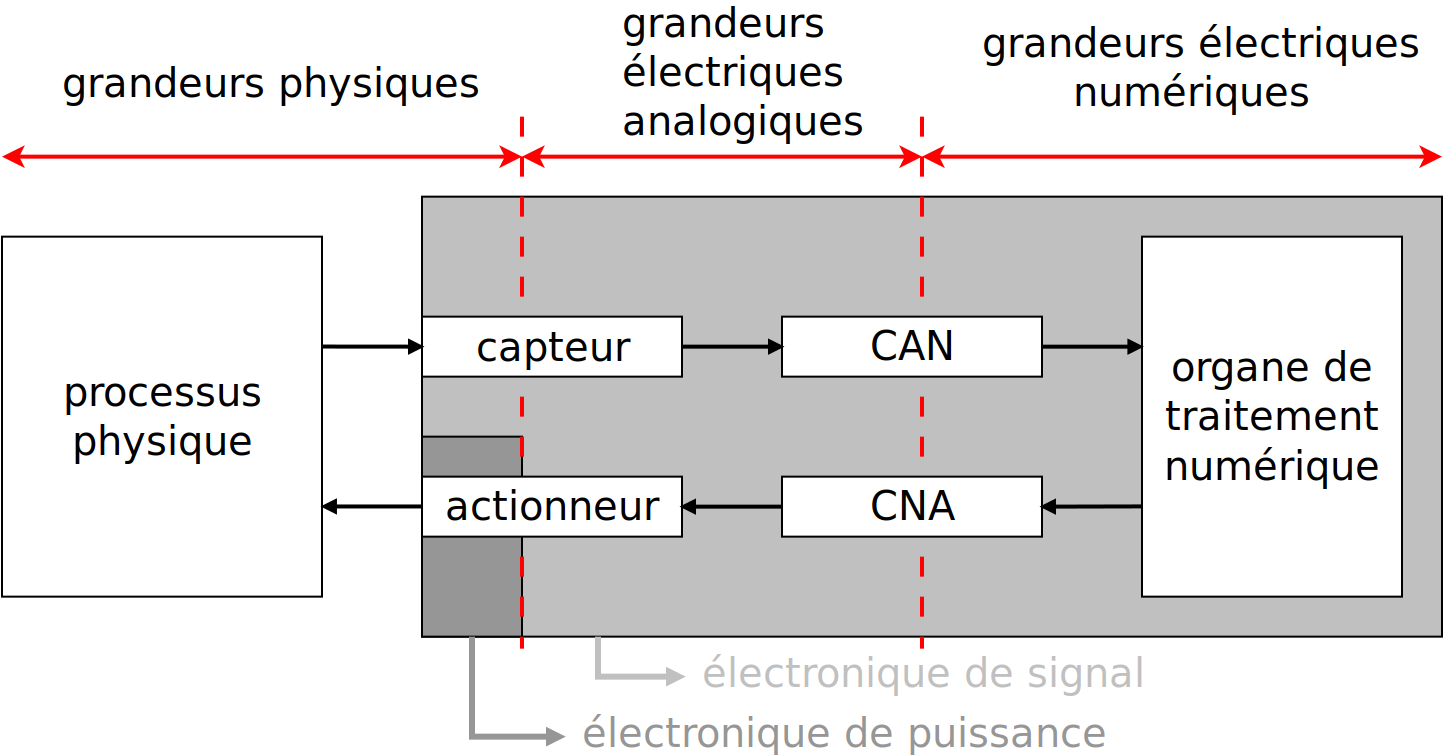
\includegraphics[width=\textwidth]{arch-processus}
	\caption{Architecture d'un processus}
	\label{fig:arch-processus}
\end{figure}

\subsection{Conversion analogique-numérique}
Le convertisseur analogique-numérique a pour rôle de transformer une tension analogique (évoluant de manière continue) en un nombre binaire codé sur un nombre de bits définis (10 ou 12 pour le dsPIC).

Pour ce faire, le convertisseur réalise une double quantification (voir figure~\ref{fig:double-quant})~:
\begin{itemize}
	\item Quantification dans le temps~: c’est l’échantillonnage.
	\item Quantification en niveau.
\end{itemize}
Il faut noter qu’il est impossible de représenter parfaitement un signal analogique sur un nombre fini de bits.


\begin{figure}[H]
	\centering
	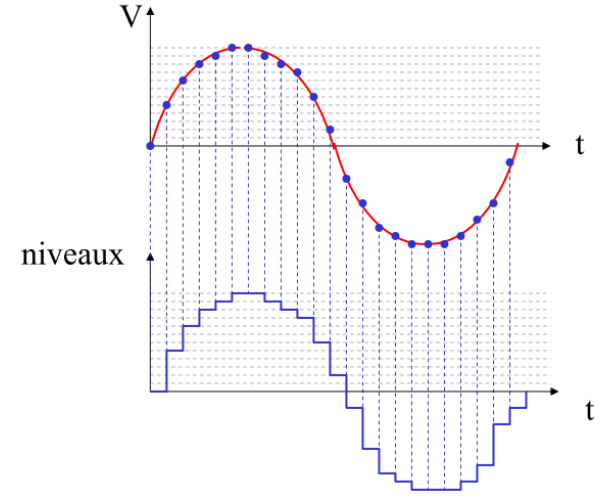
\includegraphics[width=.7\textwidth]{double-quant}
	\caption{Double quantification}
	\label{fig:double-quant}
\end{figure}

Le rendu d’un convertisseur numérique-analogique dépend donc essentiellement de deux paramètres~:
\begin{itemize}
	\item La fréquence d’échantillonnage.
	\item La résolution, c’est-à-dire le nombre de bits N codant la grandeur convertie.
	La résolution peut également être définie électriquement comme étant la plus petite variation de tension détectable.
	Si le convertisseur a une plage de fonctionnement de 0~V à 5~V et convertit la grandeur sur 10 bits, la résolution est de $\frac{5 V}{2^{10}} = 4,9 mV$(\textit{i.e.} plage d’entrée / étendue des codes binaires).
	Au final, à chaque code binaire sur N bits correspondra à une plage de tension d’entrée.
\end{itemize}

\begin{figure}
	\centering
	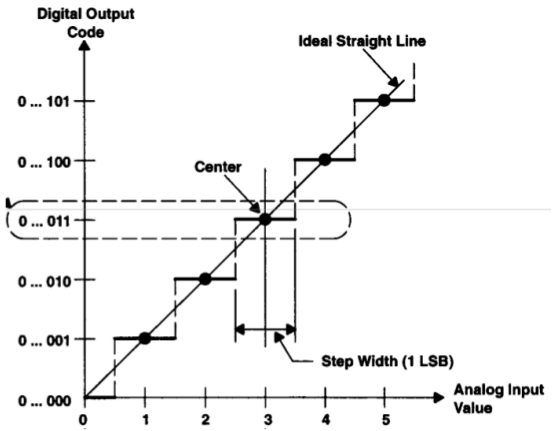
\includegraphics[width=.7\textwidth]{an-dig}
	\caption{Codage numérique d'une valeur analogique}
	\label{fig:an-dig}
\end{figure}

\subsection{Conversion numérique-analogique}
Son principe est l’inverse du CAN~: il transforme un nombre codé sur N bits en une tension comprise dans sa plage de sortie.
La tension obtenue est continue dans le temps (le convertisseur garde sa sortie constante tant qu’une nouvelle conversion n’est pas effectuée), mais elle est toujours quantifiée sur sa valeur car seules $2^N$ tensions différentes sont réalisables (chaque code binaire correspond à une tension).













\section{Prédéterminations}\label{sec:predet}
\begin{enumerate}
	\item Calculez la résolution du CAN se trouvant sur la carte Explorer16 sachant que la plage de tension d’entrée est de 0/3,3V et qu’il comporte 12bits.
	\item Déterminez l’espace mémoire nécessaire au stockage d’un fichier sonore de 3s, échantillonné à 11kHz, en sachant que chaque échantillon est stocké sur un octet.
\end{enumerate}













\section{Manipulation}

\subsection{Réalisation d'un voltmètre}
Dans un premier temps, vous allez vous familiariser avec l’utilisation du convertisseur analogique-numérique à l’aide d’une application simple~: un voltmètre mesurant la tension à la sortie d’un potentiomètre connecté à l’entrée \texttt{AN0}.
Un retour visuel se fera en utilisant les LED comme bargraph (plus la tension est élevée, plus le nombre de LED allumées doit être élevé).
Le bargraph devra être rafraichi à une cadence de 1~kHz.
\begin{itemize}
	\item Tracez le schéma bloc complet de votre système.
	Quels périphériques allez-vous utiliser~?
	Mettez en évidence les interfaces entre l’intérieur et l’extérieur du $\mu$C et indiquez clairement en encadrant les blocs internes au $\mu$C.
	\item Programmez l’ADC1 du dsPIC. Quelques lignes de code ont déjà été écrites pour mettre l’ADC dans un état de fonctionnement normal.
	Créez également une base de temps à la bonne fréquence. Pour lier les deux, vous avez le choix entre plusieurs implémentations~:
	\begin{itemize}
		\item Tester le bit de flag du timer pour lancer la conversion, et tester ensuite le bit de fin de conversion (\texttt{IFS0bits.AD1IF})
		\item Configurer l’ADC de sorte à ce que le débordement du timer lance automatiquement la conversion.
		Ceci se fait en modifiant le champ \texttt{AD1CON1bits.SSRC} (cf. figure 32 dans la section 11 du guide de programmation).
		Note~: dans tous les cas, votre fonction ne peut pas être bloquante.
	\end{itemize}
	\item Réalisez le traitement de l’information en provenance de l’ADC\footnote{érifiez la connection du potentiomètre, voir figure~\ref{fig:extension-board-jumper}}.
	\item Parmi les choix d’implémentation, lesquels garantissent la période d’échantillonnage~?
\end{itemize}

\begin{figure}[h]
\centering
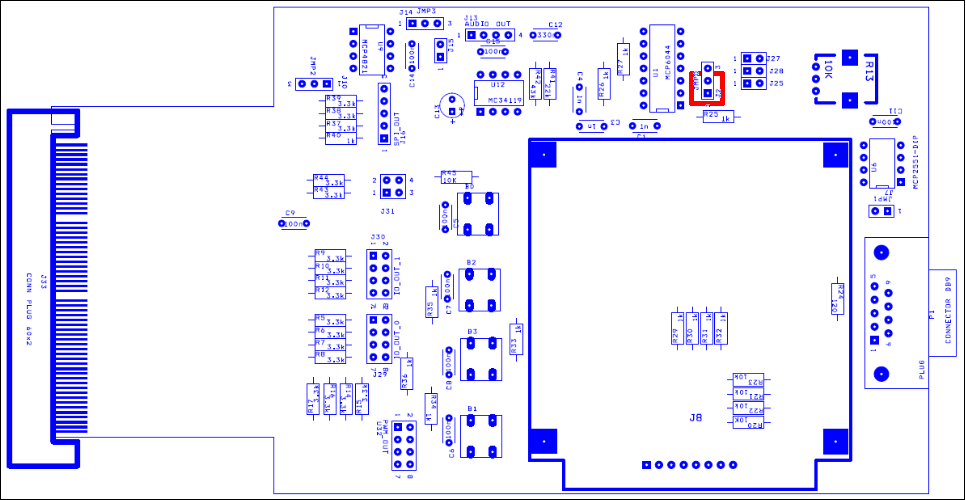
\includegraphics[width=0.9\textwidth]{extension-board-jumper}
\caption{Connectez les pattes 1 et 2 du header \texttt{J2} à l'aide d'un jumper afin de connecter le potentiomètre à l'entrée de l'ADC.}
\label{fig:extension-board-jumper}
\end{figure}

\subsection{Synthétiseur}
Un synthétiseur est un appareil capable de générer une onde sonore arbitraire et de faire jouer ce son par des baffles.
Dans notre cas, nous allons nous satisfaire d’un simple sinus de fréquence réglable~: le processeur devra envoyer un à un des échantillons correspondant à la forme d’onde voulue vers un convertisseur numérique-analogique et, une fois l’onde reconstruite, la faire passer dans l’amplificateur audio de la carte d’extension.
\begin{itemize}
	\item Vérifiez que la ligne de code appelant \texttt{clav2LCD} est mise en commentaire.
	\item Lors de la configuration de vos périphériques (avant la boucle while), remplissez le vecteur wave défini en variable globale pour qu’il contienne une période complète de sinus compris entre -2000 et 2000.
	Pour ce faire, vous devrez
	\begin{itemize}
		\item inclure le fichier math.h dans l’entête~;
		\item appeler la fonction sin() , prenant pour paramètre un nombre flottant représentant l’angle en radians et renvoyant également un flottant.
	\end{itemize}
	\item Programmez un timer pour qu’il traite un échantillon du sinus toutes les 50~$\mu$s
	\item Faites jouer le son par le baffle. Le convertisseur numérique-analogique est externe au contrôleur et s’accède via la fonction \texttt{ecrit\_dac\_signal()}, définie dans CNAserie.h et prenant en paramètre un entier un nombre compris entre 0 et 4095 (vous devrez donc recentrer votre sinus autour de 2048).
	À l’aide de l’oscilloscore, vérifiez la forme d’onde.
	\item Décommentez la ligne faisant l’appel à clav2LCD.
	Pour quelle raison votre programme ne fonctionne-t-il plus correctement~?
	\item Modifiez votre programme pour que le traitement soit réalisé dans la routine d’interruption du timer.
	En quoi cela corrige-t-il le problème~?
	\item Ajoutez un contrôle du volume en couplant la mesure du potentiomètre (représentant le volume) et votre synthétiseur.
\end{itemize}



\end{document}
